\documentclass[10pt,serif,t]{beamer}

\usepackage{graphicx}

% Environment for a slide
\newenvironment{Slide}[1]
{
  \begin{frame}[fragile,environment=Slide]
    \frametitle{#1}
    \section{#1}
  }
  {
  \end{frame}
}

% Environment for a sub slide
\newenvironment{SubSlide}[1]
{
  \begin{frame}[fragile,environment=SubSlide]
    \frametitle{#1}
    \subsection{#1}
  }
  {
  \end{frame}
}

% Environment for a sub sub slide
\newenvironment{SubSubSlide}[1]
{
  \begin{frame}[fragile,environment=SubSubSlide]
    \frametitle{#1}
    \subsubsection{#1}
  }
  {
  \end{frame}
}

% \usetheme{Hannover}
% \usetheme{Montpellier}

\title{Cost effective, large scale, fixed world 3D scanning}
% \subtitle{SUBTITLE}
\author{Dan Nixon (120263697)}
\date{March 2017}

\setbeamerfont{caption}{size=\scriptsize}

\begin{document}

\frame{\titlepage}

\begin{Slide}{3D scanning}
  \begin{itemize}
    \item
      Growing in popularity

      \begin{itemize}
        \item
          Equipment is getting cheaper

        \item
          Scan fidelity is improving

      \end{itemize}

    \pause

    \item
      More uses are always being found

  \end{itemize}

  \vspace{1em}

  \pause

  Large scale 3D scanning goals:

  \begin{itemize}
    \item
      Low cost

    \item
      Physically unlimited world size (at least up to building scale)

    \item
      Computational complexity that allows scalability

    \item
      Works regardless of mounting system/vehicle

  \end{itemize}
\end{Slide}

\begin{SubSlide}{Moving world}
  \begin{itemize}
    \item
      Move the world being scanned around a fixed sensor

    \item
      Know to a high accuracy the orientation of the world

    \item
      Limited world size

      \vspace{1em}

      \pause

    \item
      Examples:

      \begin{itemize}
        \item
          DAVID 3D (\url{http://www.david-3d.com})

        \item
          FabScan (\url{https://hci.rwth-aachen.de/fabscan})

      \end{itemize}

  \end{itemize}

  \begin{figure}
    \centering
    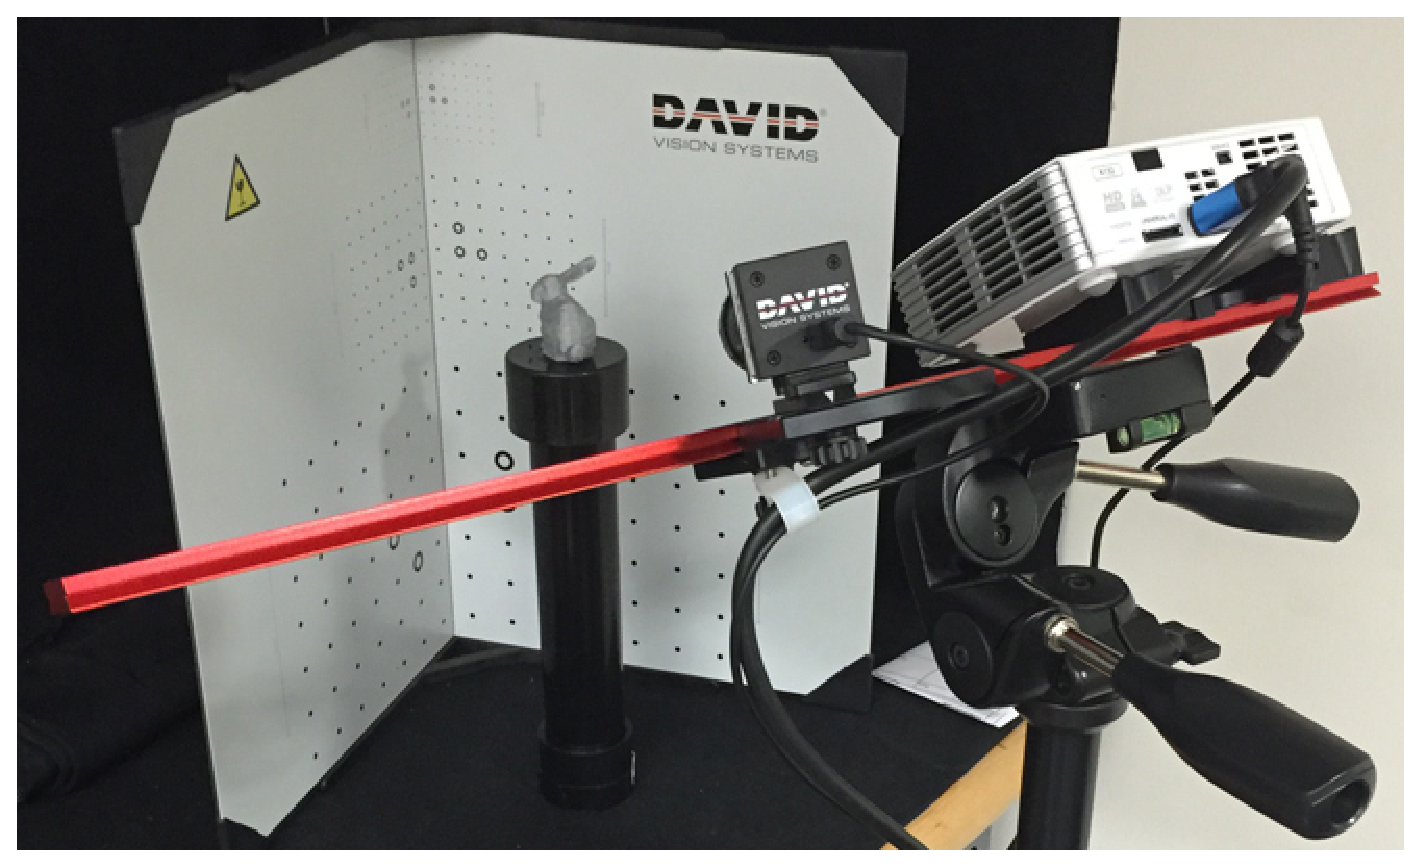
\includegraphics[height=3.5cm]{graphics/DAVID_SLS_Scanner.eps}
    \caption{DAVID SLS scanner (\url{https://productrealization.stanford.edu})}
    \label{fig:VisualSFM_Demo}
  \end{figure}
\end{SubSlide}

\begin{SubSlide}{Moving sensor}
  \begin{itemize}
    \item
      Moving sensor in a fixed world

    \item
      No physical limit to world size

    \item
      Well suited to large scale objects/environment scanning

      \vspace{1em}

      \pause

    \item
      Examples:

      \begin{itemize}
        \item
          VisualSFM (\url{http://ccwu.me/vsfm})

        \item
          Autodesk 123D Catch (\url{http://www.123dapp.com/catch})

      \end{itemize}

  \end{itemize}

  \pause

  \begin{figure}
    \centering
    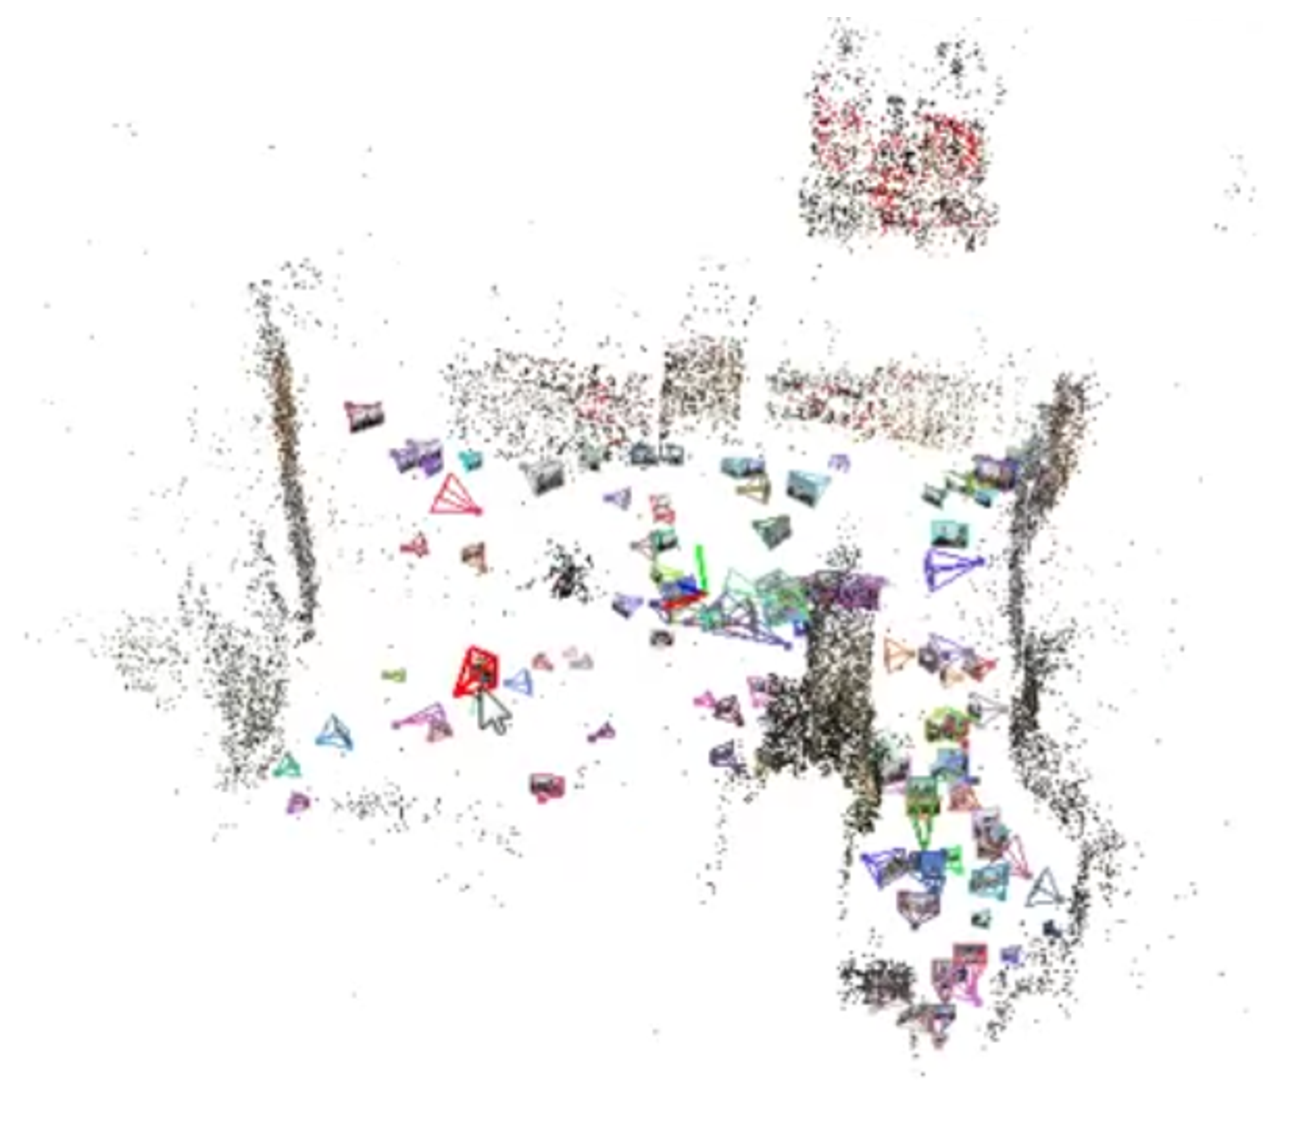
\includegraphics[height=3.5cm]{graphics/VisualSFM_Demo.eps}
    \caption{VisualSFM 3D reconstruction (\url{http://ccwu.me/vsfm/\#demo})}
    \label{fig:VisualSFM_Demo}
  \end{figure}
\end{SubSlide}

\begin{SubSlide}{Simultaneous localisation and mapping (SLAM)}
  \begin{itemize}
    \item
      Problem of mapping an unknown environment whilst keeping track of location
      within environment

      \vspace{1em}

      \pause

    \item
      No "general" solution exists, often solution is dependant on the desired
      application

    \item
      3D environment scanning can be performed as a primary function or obtained
      as "by-product" data

      \begin{itemize}
        \item
          The imaging data may be used to assist with position sensing

      \end{itemize}

      \vspace{1em}

      \pause

    \item
      Examples:

      \begin{itemize}
        \item
          Kintinuous (\url{http://www.cs.nuim.ie/research/vision/data/rgbd2012})

        \item
          Google Project Tango (\url{https://developers.google.com/tango})

      \end{itemize}

  \end{itemize}
\end{SubSlide}

\begin{Slide}{Pure positional scanning}
  \begin{itemize}
    \item
      Hypothesis: given a sufficiently accurate sensor position and orientation,
      alignment of captured point clouds on a large scale becomes trivial

      \vspace{1em}

      \pause

    \item
      Given approximate position and orientation of the sensor in each "frame",
      generation of a point cloud that reconstructs the world could be done
      though a series of transformations and pairwise alignment of point clouds

    \item
      Transformed clouds should only require pairwise alignment into a "global"
      point cloud

      \vspace{1em}

      \pause

    \item
      Measuring accurate orientation is relatively straightforward

    \item
      Measuring accurate position in non trivial

  \end{itemize}
\end{Slide}

\begin{SubSlide}{Position sensing}
  \begin{itemize}
    \item
      Double integral of acceleration

      \begin{itemize}
        \item
          Precise

        \item
          Very prone to drift over time

      \end{itemize}

      \pause

    \item
      GPS

      \begin{itemize}
        \item
          Accurate

        \item
          Low precision

        \item
          Absolute

      \end{itemize}

      \pause

    \item
      Sonar altitude

      \begin{itemize}
        \item
          Accurate

        \item
          Limited range (with low cost devices)

      \end{itemize}

    \item
      Barometric altitude

      \begin{itemize}
        \item
          Low precision

        \item
          Wide range

      \end{itemize}

  \end{itemize}
\end{SubSlide}

\begin{SubSlide}{Data Fusion}
  \begin{itemize}
    \item
      Use a combination of each measurement to determine the most likely
      position

    \item
      Each measurement has a given error

      \vspace{1em}

      \pause

    \item
      Representing sensor error as a Gaussian function:

  \end{itemize}

  \begin{figure}
    \centering
    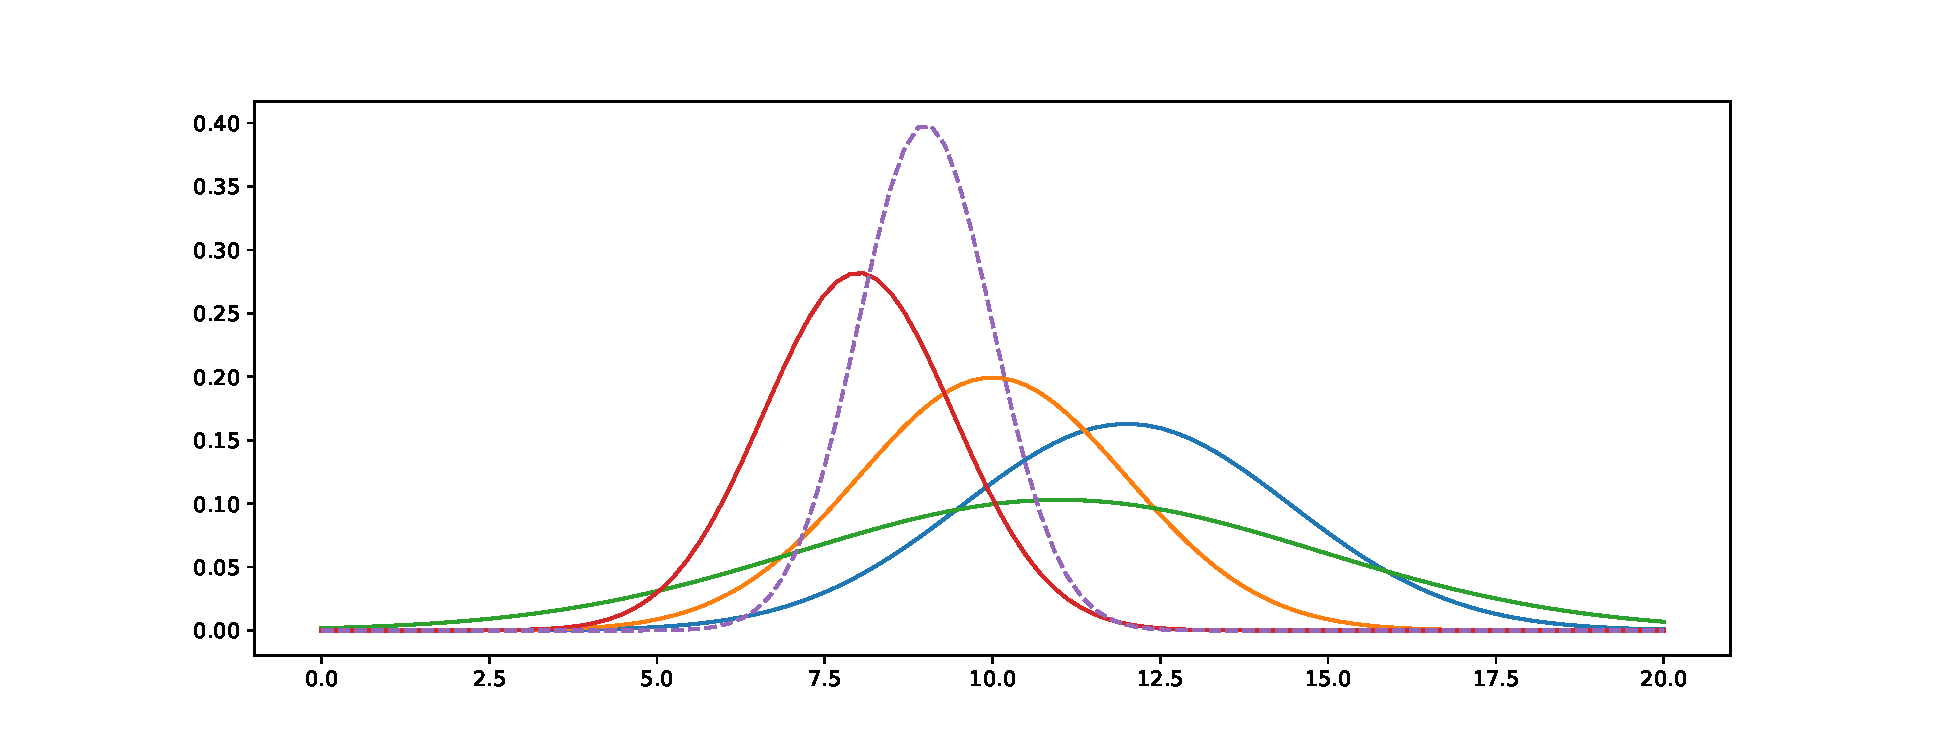
\includegraphics[height=4cm]{graphics/gaussians.eps}
    \caption{Error distribution of several position sensors}
    \label{fig:VisualSFM_Demo}
  \end{figure}
\end{SubSlide}

\begin{SubSubSlide}{Kalman filter}
  \begin{itemize}
    \item
      Very common data fusion algorithm

      \vspace{1em}

      \pause

    \item
      Model:
      \begin{align*}
        x_{t} &= F_{t}x_{t-1} + B_{t}u_{t} + w_{t} \\
        z_{t} &= H_{t}x_{t} + v_{t}
      \end{align*}

    \item
      Time update:
      \begin{align*}
        \hat{x}^{-}_{t} &= F_{t}x_{t-1}m + B_{t}u_{t} \\
        P^{-}_{t} &= F_{t}P_{t-1}F_{t}^{T} + Q
      \end{align*}

    \item
      Measurement update:
      \begin{align*}
        K_{t} &= P^{-}_{t}H^{T}(HP^{-}_{t}H^{T} + R)^{-1}\\
        \hat{x}_{t} &= \hat{x}^{-}_{t} + K_{t}(z_{t} - H\hat{x}^{-}_{t}) \\
        P_{t} &= (I-K_{t}H)P^{-}_{k}
      \end{align*}

  \end{itemize}
\end{SubSubSlide}

\begin{SubSlide}{Pairwise point cloud alignment}
  The PCL way (\url{http://pointclouds.org/documentation})

  \vspace{1em}

  \pause

  \begin{itemize}
    \item
      Generate a list of keypoints from both point clouds

      \begin{itemize}
        \item
          A point in the scene that has a special property that makes it
          identifiable with respect to it's surroundings

      \end{itemize}

      \pause

    \item
      From all pairs of keypoints, generate a list of features descriptors

      \pause

    \item
      Find correspondences between features

      \begin{itemize}
        \item
          Find overlaps in the point clouds based on similar features

      \end{itemize}

      \pause
  \end{itemize}

  \begin{figure}
    \centering
    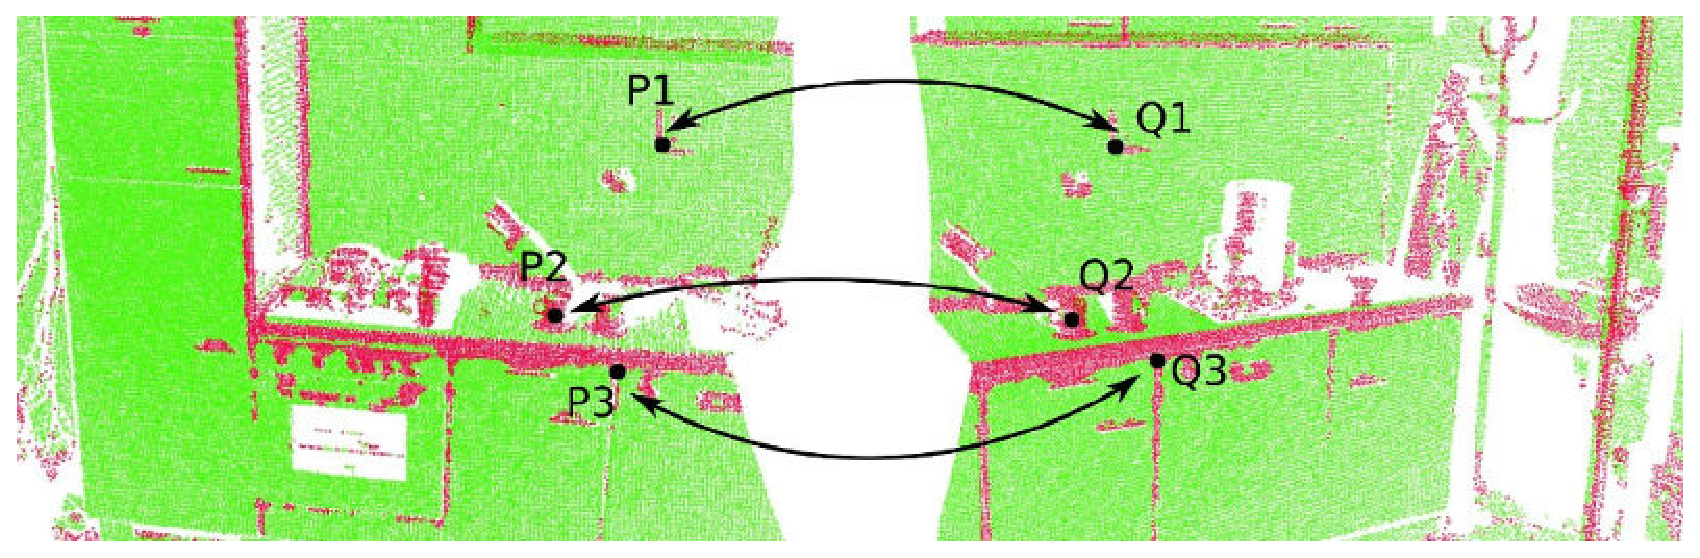
\includegraphics[height=2.5cm]{graphics/pcl_features.eps}
    \caption{Feature finding in PCL (\url{http://www.pointclouds.org/documentation})}
    \label{fig:pcl_features}
  \end{figure}
\end{SubSlide}

\begin{SubSlide}{Pairwise point cloud alignment}
  \begin{itemize}
    \item
      Reject bad correspondences

      \begin{itemize}
        \item
          Identify and remove correspondences that do not represent overlap in
          point clouds

        \item
          Such correspondences negatively effect calculation of alignment

      \end{itemize}

      \pause

    \item
      Transformation estimation

      \begin{itemize}
        \item
          Evaluate correctness of camera transformation using a metric of
          correspondences

        \item
          Optimise correctness function to obtain the optimal camera transform

        \item
          Invert transformation to obtain relative transformation between point
          clouds

      \end{itemize}

  \end{itemize}
\end{SubSlide}

\begin{Slide}{Proposed workflow}
  \begin{enumerate}
    \item[1]
      Capture point clouds

      \begin{itemize}
        \item
          Point clouds obtained through off the shelf depth sensor

        \item
          Approximate sensor position and orientation captured from IMU

      \end{itemize}

    \item[2]
      Transform point clouds by IMU data

    \item[3]
      Incrementally align point clouds into a large "world" point cloud

    \item[4]
      Triangulate a mesh from the point cloud

  \end{enumerate}
\end{Slide}

\begin{Slide}{Conclusion}
  \begin{itemize}
    \item
      Camera pose based scanner is possible if pose is accurate and precise

    \item
      Sensor fusion could provide a sufficiently accurate position

    \item
      Combination of commodity RGB-D camera and sensors

    \item
      Operates in areas of few distinct features

  \end{itemize}
\end{Slide}

\end{document}
